\section{Results and Discussion}

Table~\ref{tab:main_results} reports the final test-set results. The strongest
overall model is the XGBoost context baseline, which uses PM2.5 history,
weather, and calendar features. It obtains MSE 26.185 and MAE 3.125. The full
Event-TimeRAF XGBoost variant obtains MSE 26.712 and MAE 3.149. Therefore, this
run does not support a claim that the full Event-TimeRAF XGBoost variant
outperforms the strongest non-retrieval context baseline on the all-origin test
set. It does, however, substantially outperform the persistence and seasonal
naive baselines.

\begin{table*}[!t]
\centering
\caption{Final Overall Test Results for 24-Hour PM2.5 Forecasting}
\label{tab:main_results}
\begin{tabular}{lrrrr}
\toprule
Model & MSE & MAE & RMSE & $R^2$ \\
\midrule
M00 persistence & 47.649 & 4.137 & 6.903 & -0.130 \\
M01 daily seasonal & 48.706 & 4.057 & 6.979 & -0.155 \\
M02 weekly seasonal & 65.606 & 5.123 & 8.100 & -0.556 \\
M03 XGBoost PM2.5 & 29.949 & 3.368 & 5.473 & 0.290 \\
M04 XGBoost context & \textbf{26.185} & \textbf{3.125} & \textbf{5.117} & \textbf{0.379} \\
M05 random retrieval & 42.367 & 4.257 & 6.509 & -0.005 \\
M06 cosine retrieval & 38.083 & 3.940 & 6.171 & 0.097 \\
M07 XGBoost cosine & 26.672 & 3.151 & 5.164 & 0.367 \\
M08 Event-TimeRAF no drift & 26.677 & 3.145 & 5.165 & 0.367 \\
M09 Event-TimeRAF full & 26.712 & 3.149 & 5.168 & 0.367 \\
M10 frozen Chronos-Bolt & 28.941 & 3.205 & 5.380 & 0.314 \\
M11 Chronos + retrieval & 28.709 & 3.209 & 5.358 & 0.319 \\
\bottomrule
\end{tabular}
\end{table*}

The frozen Chronos-Bolt publication gate completed successfully. The validation
fusion search selected a retrieval-fusion weight of 0.75. On the test set,
retrieval-augmented Chronos reduces MSE from 28.941 to 28.709, an improvement of
about 0.8\% relative to frozen Chronos-Bolt. The paired block-bootstrap
comparison gives an MSE difference of -0.233 with a 95\% interval from -0.665 to
0.152, so the direction is favorable but not conclusive under this uncertainty
estimate. MAE changes from 3.205 to 3.209, which is practically flat.

Table~\ref{tab:ablation_results} summarizes the main ablation comparisons. The
clearest supported gain is from adding weather and calendar context to the
PM2.5-only XGBoost model: MSE decreases by 3.764 and the confidence interval is
fully below zero. Cosine retrieval improves over random retrieval in the
retrieval-only setting. In contrast, adding cosine retrieval features to the
already strong XGBoost context model does not improve the all-origin result in
this run. Event-hybrid retrieval and drift indicators also do not show a clear
overall improvement beyond the context baseline.

\begin{table*}[!t]
\centering
\caption{Selected Paired Block-Bootstrap Ablation Results}
\label{tab:ablation_results}
\begin{tabular}{lrrr}
\toprule
Comparison & MSE diff. & 95\% CI low & 95\% CI high \\
\midrule
M04 minus M03, weather/calendar & -3.764 & -5.856 & -2.071 \\
M06 minus M05, cosine/random retrieval & -4.284 & -5.862 & -2.759 \\
M07 minus M04, retrieval features & 0.487 & 0.015 & 1.028 \\
M08 minus M07, event hybrid & 0.005 & -0.292 & 0.275 \\
M09 minus M08, drift indicators & 0.035 & -0.101 & 0.161 \\
M09 minus M04, full Event-TimeRAF & 0.528 & -0.026 & 1.182 \\
M11 minus M10, Chronos retrieval & -0.233 & -0.665 & 0.152 \\
\bottomrule
\end{tabular}
\end{table*}

The $k$ sensitivity results in Table~\ref{tab:k_sensitivity} show that the
retrieval-only cosine baseline improves as more neighbors are used within the
tested range. The best retrieval-only configuration among $k \in \{1,4,8,16\}$
is $k=16$, with MSE 36.488. The final Event-TimeRAF feature models used the
pre-specified default $k=8$.

\begin{table}[!t]
\centering
\caption{Cosine Retrieval Sensitivity to $k$}
\label{tab:k_sensitivity}
\begin{tabular}{rrrr}
\toprule
$k$ & MSE & MAE & RMSE \\
\midrule
1 & 65.129 & 5.133 & 8.070 \\
4 & 41.237 & 4.134 & 6.422 \\
8 & 38.083 & 3.940 & 6.171 \\
16 & 36.488 & 3.851 & 6.040 \\
\bottomrule
\end{tabular}
\end{table}

Fig.~\ref{fig:mse_horizon} and Fig.~\ref{fig:mae_horizon} show horizon-wise
test errors. Fig.~\ref{fig:retrieval_diagnostics} summarizes retrieval behavior,
and Fig.~\ref{fig:drift_scores} shows the drift-score distribution across the
test period. These plots are generated directly from the saved final-run
artifacts and share run identifier \texttt{20260723T112033170131Z}.

\begin{figure}[!t]
\centering

\includegraphics[width=\columnwidth]{figures/mse_by_horizon.png}
\caption{MSE by forecast horizon for the final test run.}
\label{fig:mse_horizon}
\end{figure}

\begin{figure}[!t]
\centering
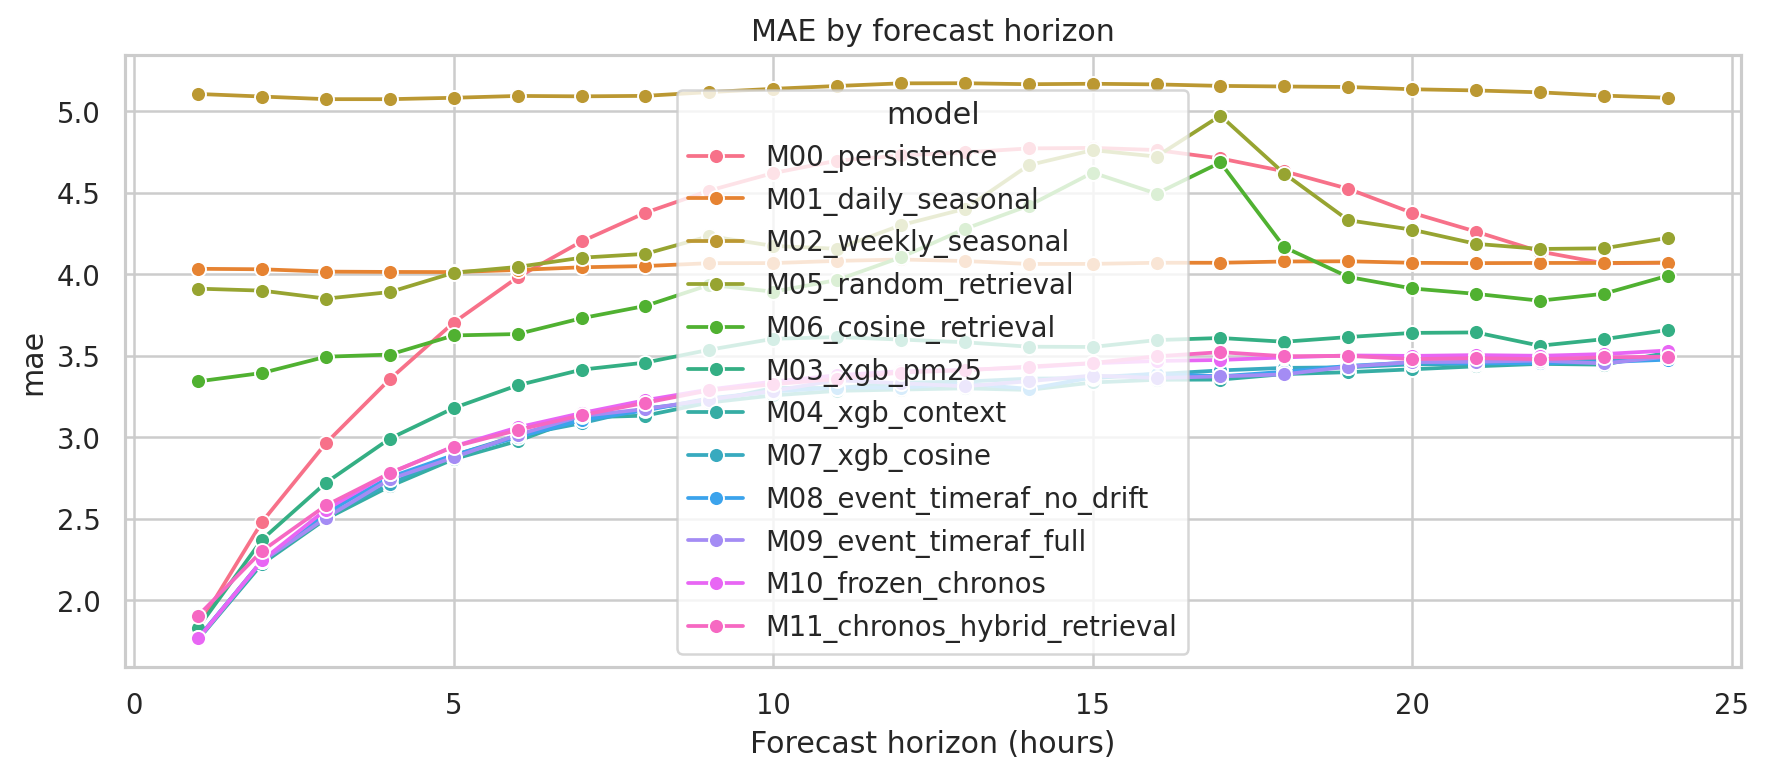
\includegraphics[width=\columnwidth]{figures/mae_by_horizon.png}
\caption{MAE by forecast horizon for the final test run.}
\label{fig:mae_horizon}
\end{figure}

\begin{figure}[!t]
\centering
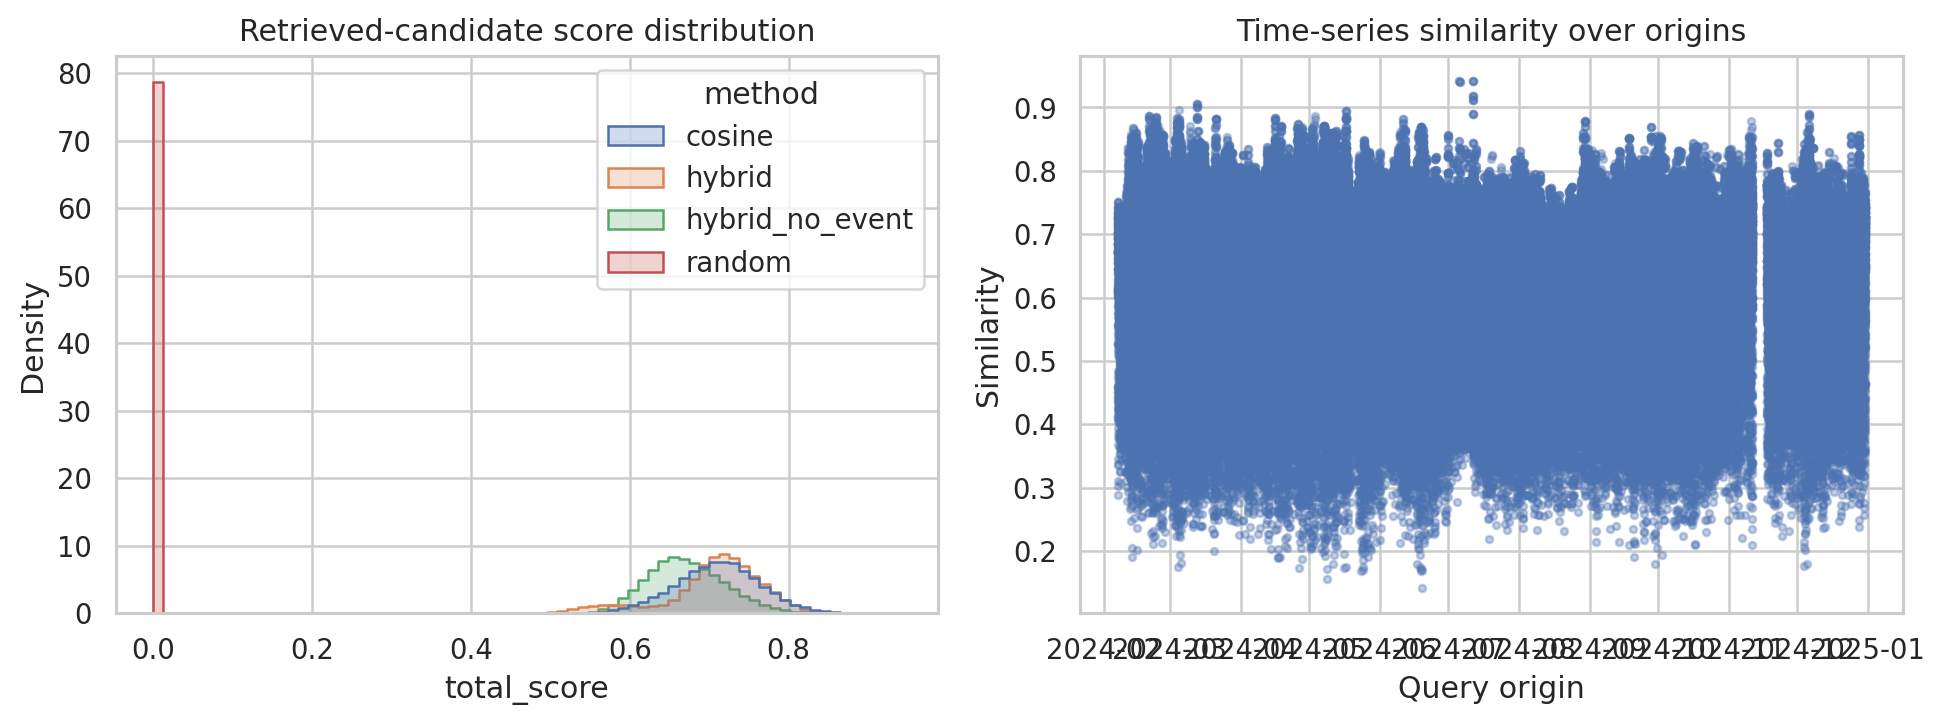
\includegraphics[width=\columnwidth]{figures/retrieval_diagnostics.png}
\caption{Retrieval diagnostics for the final test run.}
\label{fig:retrieval_diagnostics}
\end{figure}

\begin{figure}[!t]
\centering
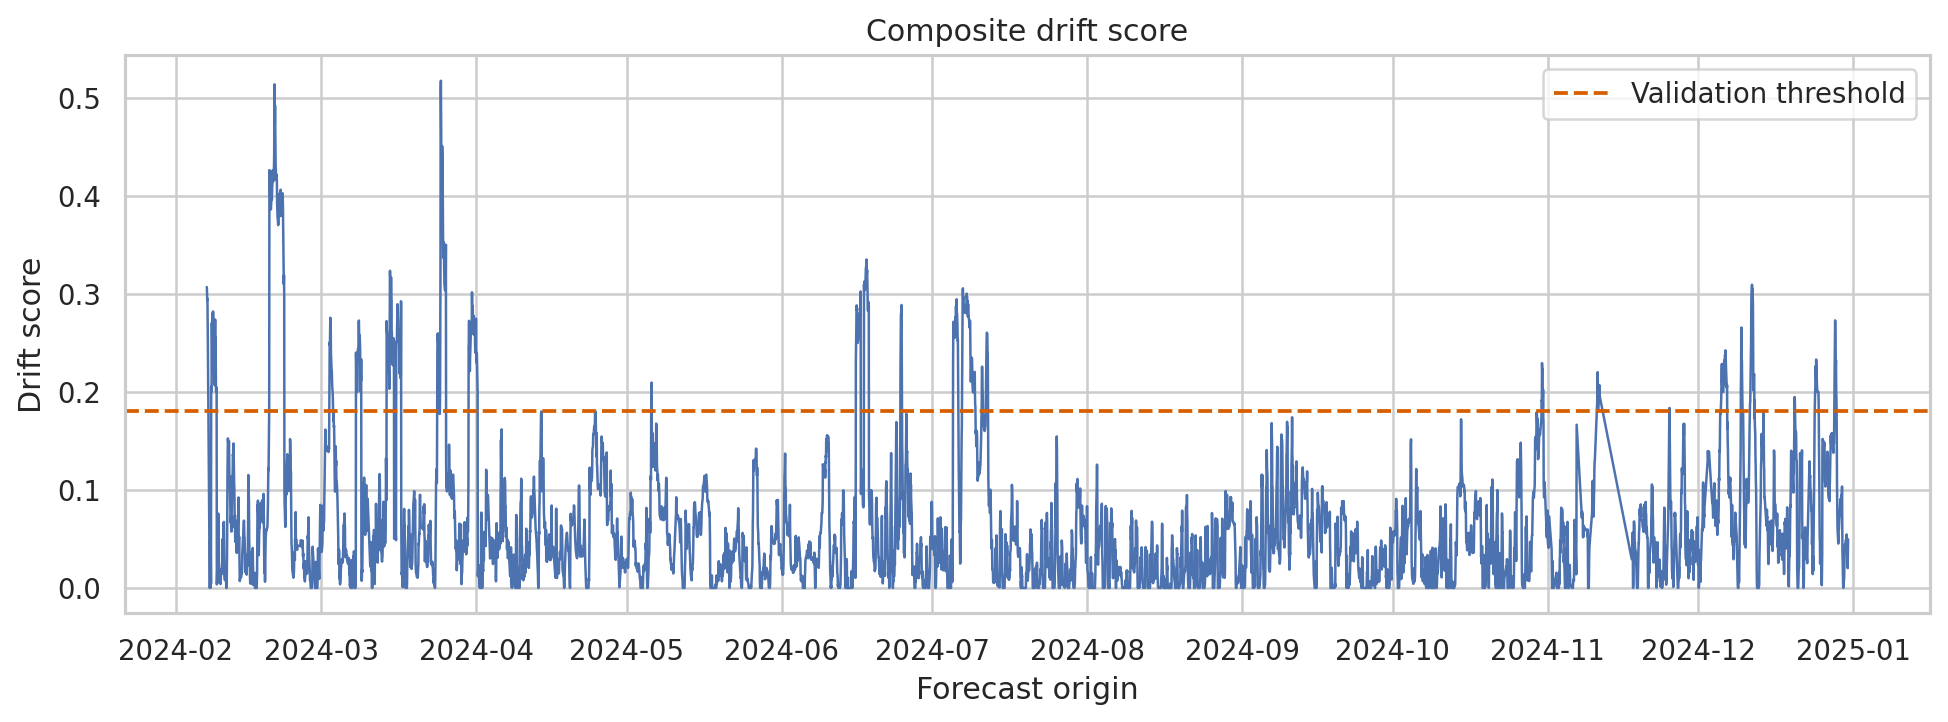
\includegraphics[width=\columnwidth]{figures/drift_scores.png}
\caption{Drift-score diagnostics for the final test run.}
\label{fig:drift_scores}
\end{figure}

The main interpretation is that conventional supervised context features are
very strong for this Los Angeles County 24-hour PM2.5 task. Retrieval is useful
as a standalone historical-pattern baseline and gives a small favorable MSE
change when fused with frozen Chronos-Bolt, but the present feature-level
Event-TimeRAF design does not beat the best XGBoost context baseline overall.
This negative result is important for the final paper: Event-TimeRAF should be
presented as an implemented and audited event-aware retrieval framework with
mixed empirical effects, not as a uniformly superior forecasting model.

Finally, all event-aware interpretations must be read with the availability
caveat. NOAA Storm Events records are official and hash-verified, but the source
does not provide machine-readable publication timestamps. The experiment records
event start as the availability time, so event-related results are retrospective
sensitivity results. A strict operational study would require event or smoke
sources with genuine issue or publication times, such as an audited NOAA HMS
cache or alert product archive.
